

\tikzset{every picture/.style={line width=0.75pt}} %set default line width to 0.75pt        

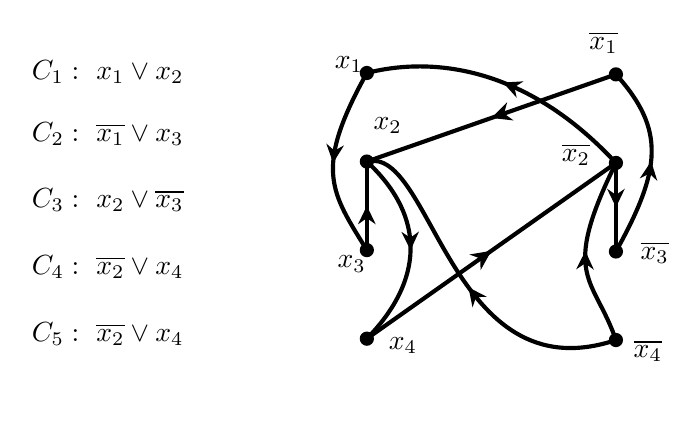
\begin{tikzpicture}[x=0.5pt,y=0.5pt,yscale=-1,xscale=1]
%uncomment if require: \path (0,248); %set diagram left start at 0, and has height of 248

%Flowchart: Connector [id:dp5285899162991353] 
\draw  [fill={rgb, 255:red, 0; green, 0; blue, 0 }  ,fill opacity=1 ] (252,32) .. controls (252,29.58) and (253.96,27.62) .. (256.38,27.62) .. controls (258.79,27.62) and (260.75,29.58) .. (260.75,32) .. controls (260.75,34.42) and (258.79,36.38) .. (256.38,36.38) .. controls (253.96,36.38) and (252,34.42) .. (252,32) -- cycle ;
%Straight Lines [id:da03484807968209058] 
\draw [color={rgb, 255:red, 0; green, 0; blue, 0 }  ,draw opacity=1 ][line width=1.5]    (256.38,224) -- (436.38,97) ;
\draw [shift={(346.38,160.5)}, rotate = 504.8] [fill={rgb, 255:red, 0; green, 0; blue, 0 }  ,fill opacity=1 ][line width=0.08]  [draw opacity=0] (14.56,-6.99) -- (0,0) -- (14.56,6.99) -- (9.67,0) -- cycle    ;
%Flowchart: Connector [id:dp28963957089609804] 
\draw  [fill={rgb, 255:red, 0; green, 0; blue, 0 }  ,fill opacity=1 ] (252,96) .. controls (252,93.59) and (253.96,91.63) .. (256.38,91.63) .. controls (258.79,91.63) and (260.75,93.59) .. (260.75,96) .. controls (260.75,98.42) and (258.79,100.38) .. (256.38,100.38) .. controls (253.96,100.38) and (252,98.42) .. (252,96) -- cycle ;
%Flowchart: Connector [id:dp5510231189769008] 
\draw  [fill={rgb, 255:red, 0; green, 0; blue, 0 }  ,fill opacity=1 ] (252,160.01) .. controls (252,157.59) and (253.96,155.63) .. (256.38,155.63) .. controls (258.79,155.63) and (260.75,157.59) .. (260.75,160.01) .. controls (260.75,162.42) and (258.79,164.38) .. (256.38,164.38) .. controls (253.96,164.38) and (252,162.42) .. (252,160.01) -- cycle ;
%Flowchart: Connector [id:dp8347416280872515] 
\draw  [fill={rgb, 255:red, 0; green, 0; blue, 0 }  ,fill opacity=1 ] (252,224) .. controls (252,221.58) and (253.96,219.62) .. (256.38,219.62) .. controls (258.79,219.62) and (260.75,221.58) .. (260.75,224) .. controls (260.75,226.42) and (258.79,228.38) .. (256.38,228.38) .. controls (253.96,228.38) and (252,226.42) .. (252,224) -- cycle ;
%Flowchart: Connector [id:dp09589448620018437] 
\draw  [fill={rgb, 255:red, 0; green, 0; blue, 0 }  ,fill opacity=1 ] (432,33) .. controls (432,30.58) and (433.96,28.62) .. (436.38,28.62) .. controls (438.79,28.62) and (440.75,30.58) .. (440.75,33) .. controls (440.75,35.42) and (438.79,37.38) .. (436.38,37.38) .. controls (433.96,37.38) and (432,35.42) .. (432,33) -- cycle ;
%Flowchart: Connector [id:dp6276853107817513] 
\draw  [fill={rgb, 255:red, 0; green, 0; blue, 0 }  ,fill opacity=1 ] (432,97) .. controls (432,94.59) and (433.96,92.63) .. (436.38,92.63) .. controls (438.79,92.63) and (440.75,94.59) .. (440.75,97) .. controls (440.75,99.42) and (438.79,101.38) .. (436.38,101.38) .. controls (433.96,101.38) and (432,99.42) .. (432,97) -- cycle ;
%Flowchart: Connector [id:dp7176343531829045] 
\draw  [fill={rgb, 255:red, 0; green, 0; blue, 0 }  ,fill opacity=1 ] (432,161.01) .. controls (432,158.59) and (433.96,156.63) .. (436.38,156.63) .. controls (438.79,156.63) and (440.75,158.59) .. (440.75,161.01) .. controls (440.75,163.42) and (438.79,165.38) .. (436.38,165.38) .. controls (433.96,165.38) and (432,163.42) .. (432,161.01) -- cycle ;
%Flowchart: Connector [id:dp8859571266882346] 
\draw  [fill={rgb, 255:red, 0; green, 0; blue, 0 }  ,fill opacity=1 ] (432,225) .. controls (432,222.58) and (433.96,220.62) .. (436.38,220.62) .. controls (438.79,220.62) and (440.75,222.58) .. (440.75,225) .. controls (440.75,227.42) and (438.79,229.38) .. (436.38,229.38) .. controls (433.96,229.38) and (432,227.42) .. (432,225) -- cycle ;
%Straight Lines [id:da9353211071842927] 
\draw [color={rgb, 255:red, 0; green, 0; blue, 0 }  ,draw opacity=1 ][line width=1.5]    (436.38,33) -- (256.38,96) ;
\draw [shift={(346.38,64.5)}, rotate = 340.71000000000004] [fill={rgb, 255:red, 0; green, 0; blue, 0 }  ,fill opacity=1 ][line width=0.08]  [draw opacity=0] (14.56,-6.99) -- (0,0) -- (14.56,6.99) -- (9.67,0) -- cycle    ;
%Straight Lines [id:da07119264102777723] 
\draw [line width=1.5]    (256.38,160.01) -- (256.38,96) ;
\draw [shift={(256.38,128)}, rotate = 450] [fill={rgb, 255:red, 0; green, 0; blue, 0 }  ][line width=0.08]  [draw opacity=0] (13.4,-6.43) -- (0,0) -- (13.4,6.44) -- (8.9,0) -- cycle    ;
%Curve Lines [id:da7435687764576437] 
\draw [line width=1.5]    (436.38,97) .. controls (371.5,27) and (303.5,20) .. (256.38,32) ;
\draw [shift={(354.76,38.88)}, rotate = 382.41999999999996] [fill={rgb, 255:red, 0; green, 0; blue, 0 }  ][line width=0.08]  [draw opacity=0] (13.4,-6.43) -- (0,0) -- (13.4,6.44) -- (8.9,0) -- cycle    ;
%Curve Lines [id:da5802575901273257] 
\draw [line width=1.5]    (256.38,96) .. controls (300.5,137) and (296.5,183) .. (256.38,224) ;
\draw [shift={(287.97,160)}, rotate = 268.81] [fill={rgb, 255:red, 0; green, 0; blue, 0 }  ][line width=0.08]  [draw opacity=0] (13.4,-6.43) -- (0,0) -- (13.4,6.44) -- (8.9,0) -- cycle    ;
%Curve Lines [id:da7175218471577676] 
\draw [line width=1.5]    (436.38,225) .. controls (420.5,179) and (395.5,180) .. (436.38,97) ;
\draw [shift={(414.3,160.68)}, rotate = 451.13] [fill={rgb, 255:red, 0; green, 0; blue, 0 }  ][line width=0.08]  [draw opacity=0] (13.4,-6.43) -- (0,0) -- (13.4,6.44) -- (8.9,0) -- cycle    ;
%Curve Lines [id:da6924159573089901] 
\draw [line width=1.5]    (256.38,32) .. controls (217.5,102) and (230.5,118) .. (256.38,160.01) ;
\draw [shift={(231.99,96.97)}, rotate = 276.2] [fill={rgb, 255:red, 0; green, 0; blue, 0 }  ][line width=0.08]  [draw opacity=0] (13.4,-6.43) -- (0,0) -- (13.4,6.44) -- (8.9,0) -- cycle    ;
%Curve Lines [id:da35461450717449705] 
\draw [line width=1.5]    (436.38,161.01) .. controls (469.12,102) and (472.5,73) .. (436.38,33) ;
\draw [shift={(461.82,95.84)}, rotate = 458.06] [fill={rgb, 255:red, 0; green, 0; blue, 0 }  ][line width=0.08]  [draw opacity=0] (13.4,-6.43) -- (0,0) -- (13.4,6.44) -- (8.9,0) -- cycle    ;
%Straight Lines [id:da1097593932252855] 
\draw [line width=1.5]    (436.38,97) -- (436.38,161.01) ;
\draw [shift={(436.38,129)}, rotate = 270] [fill={rgb, 255:red, 0; green, 0; blue, 0 }  ][line width=0.08]  [draw opacity=0] (13.4,-6.43) -- (0,0) -- (13.4,6.44) -- (8.9,0) -- cycle    ;
%Curve Lines [id:da37464522628067776] 
\draw [line width=1.5]    (436.38,225) .. controls (316.5,265) and (303.5,84) .. (256.38,96) ;
\draw [shift={(329.81,186.93)}, rotate = 412.86] [fill={rgb, 255:red, 0; green, 0; blue, 0 }  ][line width=0.08]  [draw opacity=0] (13.4,-6.43) -- (0,0) -- (13.4,6.44) -- (8.9,0) -- cycle    ;

% Text Node
\draw (12,21) node [anchor=north west][inner sep=0.75pt]   [align=left] {$\displaystyle C_{1} :\ x_{1} \lor x_{2}$};
% Text Node
\draw (12,65.25) node [anchor=north west][inner sep=0.75pt]   [align=left] {$\displaystyle C_{2} :\ \overline{x_{1}} \lor x_{3}$};
% Text Node
\draw (12,113.5) node [anchor=north west][inner sep=0.75pt]   [align=left] {$\displaystyle C_{3} :\ x_{2} \lor \overline{x_{3}}$};
% Text Node
\draw (12,161.75) node [anchor=north west][inner sep=0.75pt]   [align=left] {$\displaystyle C_{4} :\ \overline{x_{2}} \lor x_{4}$};
% Text Node
\draw (12,210) node [anchor=north west][inner sep=0.75pt]   [align=left] {$\displaystyle C_{5} :\ \overline{x_{2}} \lor x_{4}$};
% Text Node
\draw (231,18) node [anchor=north west][inner sep=0.75pt]   [align=left] {$\displaystyle x_{1}$};
% Text Node
\draw (259,62) node [anchor=north west][inner sep=0.75pt]   [align=left] {$\displaystyle x_{2}$};
% Text Node
\draw (233,162) node [anchor=north west][inner sep=0.75pt]   [align=left] {$\displaystyle x_{3}$};
% Text Node
\draw (270,221) node [anchor=north west][inner sep=0.75pt]   [align=left] {$\displaystyle x_{4}$};
% Text Node
\draw (415,0) node [anchor=north west][inner sep=0.75pt]   [align=left] {$\displaystyle \overline{x_{1}}$};
% Text Node
\draw (395,81) node [anchor=north west][inner sep=0.75pt]   [align=left] {$\displaystyle \overline{x_{2}}$};
% Text Node
\draw (452,152) node [anchor=north west][inner sep=0.75pt]   [align=left] {$\displaystyle \overline{x_{3}}$};
% Text Node
\draw (447,223) node [anchor=north west][inner sep=0.75pt]   [align=left] {$\displaystyle \overline{x_{4}}$};


\end{tikzpicture}

